\chapter{运动定律}\label{chapter-law-of-motion}


% 
前一章我们学习了怎样描述物体的运动,但是没有进一步讨论物体为什么做这种或那种运动.要讨论这个问题,必须知道运动和力的关系.这一章我们就来研究运动和力的关系,阐明力是使物体运动状态发生改变的原因.在力学中,只研究物体怎样运动而不涉及运动和力的关系的分科,叫做\textbf{运动学};研究运动和力的关系的分科,叫做\textbf{动力学}.

根据动力学的知识,如果知道了物体的受力情况,就可以确定物体的运动状况;或者反过来,如果知道了物体的运动状况,也可以确定物体的受力情况.这样,我们就不但能够描述运动,而且能够创造条件来控制物体的运动,使物体的运动符合人们的要求.

动力学的知识在生产和科学研究中是很重要的.设计各种机器,控制交通工具的速度,研究天体的运动,计算人造卫星的轨道等等,都离不开动力学的知识.

动力学的奠基人是英国科学家牛顿.牛顿在1687年出版了他的名著《自然哲学的数学原理》.在这部著作中,牛顿提出了三条运动定律,这三条定律总称为牛顿运动定律,是整个动力学的基础.这一章我们学习的就是牛顿运动定律.

\section{牛顿第一定律}
在初中我们已经学过了牛顿第一定律,这一节我们先回顾一下历史,然后对这个定律本身作一些讨论.

\subsection{历史的回顾} 
远在两千多年以前,人们已经提出了运动和力的关系问题,可是直到伽利略和牛顿(1642$\sim$1727)时代,才对这个问题给出了正确的答案.

在十七世纪以前,人们普遍认为力是维持物体运动的原因.用力推车,车子才前进,停止用力,车子就要停下来.
古希腊的哲学家亚里士多德(公元前384$\sim$322)根据这类经验事实得出结论说:必须有力作用在物体上,物体才能运动
,没有力的作用,物体就要静止下来.

在亚里士多德以后的两千年内,动力学一直没有多大进展.
直到十七世纪,意大利的著名物理学家伽利略才根据实验揭示了现象的本质,指出了亚里士多德的观点的错误.
伽利略发现运动物体所以会停下来,是因为受到摩擦阻力的缘故.他断言:一旦物体具有某一速度,只要没有加速或减速的原因,这个速度将保持不变,而这种情况只有在摩擦力极小的水平面上才能近似达到.
根据这种观点看来,力不是维持物体的运动即维持物体的速度的原因,而是改变物体运动状态即改变物体速度的原因.

伽利略是怎样得到这个结论的呢?伽利略并没有脱离日常经验,而是对经验进行了分析.他研究了物体在斜面上的运动,发现物体沿斜面向下运动,有加速的原因出现,速度不
断增加,沿斜面向上运动,有减速的原因出现,速度不断减小.他根据这一事实进行推论,指出在没有倾斜的光滑水平面上,物体的运动应当是既没有加速也没有减速,速度应当是不变的.当然伽利略知道,由于物体受到摩擦力的阻碍,这种水平运动的速度实际上并不是不变的,摩擦越小,物体以接近于恒定速度运动的时间就越长.在没有摩擦的理想情况下,物体将以恒定的速度持续运动下去.

我们可以用现代的实验设备来近似地验证上述结论.把
物体放在一个水平导轨上,并设法使物体和导轨之间形成气层,物体沿这种气垫导轨运动时摩擦很小.推动一下物体,可以看到物体沿气垫导轨的运动很接近匀速直线运动.

\begin{figure}[htp]
    \centering
    \begin{subfigure} {1\linewidth} 
		\centering
		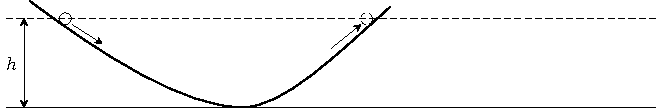
\includegraphics{fig/A/3-1a.pdf} 
		\caption{}\label{fig_A_3-1a} 
	\end{subfigure}
	\\
	\begin{subfigure} {1\linewidth} 
		\centering
		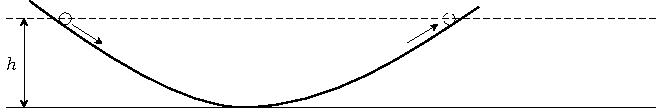
\includegraphics{fig/A/3-1b.pdf} 
		\caption{}\label{fig_A_3-1b} 
	\end{subfigure}
	\\
	\begin{subfigure} {1\linewidth} 
		\centering
		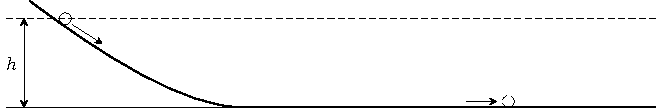
\includegraphics{fig/A/3-1c.pdf} 
		\caption{}\label{fig_A_3-1c} 
	\end{subfigure}
    \caption{伽利略的斜面实验}\label{fig_A_3-1}
\end{figure}

伽利略还根据下面的理想实验进行推论.如图~\ref{fig_A_3-1a} 所示,
让小球沿一个斜面从静止滚下来,小球将滚上另一个斜面.
如果没有摩擦,小球将上升到原来的高度.他推论说,
如果减小第二个斜面的倾角(图~\ref{fig_A_3-1b}),小球在这个斜面上达
到原来的高度就要通过更长的距离.
继续减小第二个斜面的倾角,
使它最终成为水平面(图~\ref{fig_A_3-1c}),小球就再也达不到原来的高度,
而要沿着水平面以恒定速度持续运动下去.

伽利略的实验虽然是想象中的理想实验,但它们是建立在可靠的事实的基础之上的.伽利略把经验事实和抽象思维结合起来,这正是他的工作的卓越之处.由于伽利略细心地研究了理想实验,才使他对动力学做出了重大贡献.
这类理想实验在真实的实验基础上,抓住主要因素,忽略次要因素,可以深入地揭示现象的本质,它是科学研究中的一种重要方法.

伽利略时代的法国科学家笛卡尔(1596$\sim$1650)进一步补充和完善了伽利略的论点,第一次明确地表述了惯性定律.笛卡尔认为:如果没有其他原因,运动的物体将继续以同一速度沿着一条直线运动,既不会停下来,也不会偏离原来的方向.这样,笛卡尔为发展动力学又迈出了重要一步.

\subsection{牛顿第一定律} 
牛顿在伽利略等人的研究基础上,并根据他自己的研究,系统地总结了力学的知识,提出了三条运动定律,其中第一条定律的内容是:

\textbf{一切物体总保持匀速直线运动状态或静止状态,直到有
外力迫使它改变这种状态为止.}

这就是\textbf{牛顿第一定律},物体的这种保持原来的匀速直线运动状态或静止状态的性质叫做\textbf{惯性},牛顿第一定律又叫做\textbf{惯性定律}.

汽车里的乘客,当汽车突然开动时,身体要向后面倾倒,这是因为汽车已经开始前进而乘客由于惯性要保持静止状态
的缘故.
当汽车突然停止时,身体要向前面倾倒,这是因为汽车已经停止而乘客由于惯性要保持原来速度前进的缘故.
一切物体都具有惯性,惯性是物体的固有性质,物体的运动并不需要力来维持.

牛顿第一定律所描述的是一种理想化的状态,即物体不受外力作用的状态.
但是,任何物体都和周围的物体有相互作用,不受外力作用的物体是不存在的.
物体受到几个力的作用,如果合力为零,即这几个力相互平衡,这时物体的运动状态并不发生改变.
我们通常所看到的匀速直线运动状态和静止状态,其实都是物体受到相互平衡的力的作用的结果.

\section*{阅读材料:爱因斯坦谈运动的问题}
有一个基本问题,几千年来都因为它太复杂而含糊不清,这就是运动的问题.……设想有一个静止的物体,没有任何运动,要改变这样一个物体的位置,必须使它受力,如推它,提它,或由其他的物体如马、蒸汽机作用于它.
我们的直觉认为运动是与推、提、拉等动作相连的,多次的经验使我们进一步深信,要使一个物体运动得愈快,必须用更大的力推它.
结论好象是很自然的:对一个物体的作用愈强,它的速度就愈大.一辆四匹马驾的车比一辆两匹马驾的车运动得快一些.这样,直觉告诉我们,速率主要是跟作用有关.

……

伽利略的发现以及他所应用的科学的推理方法是人类思想史上最伟大的成就之一,而且标志着物理学的真正开端.这
个发现告诉我们,根据直接观察所得出的直觉的结论不是常常可靠的,因为它们有时会引到错误的线索上去.

但是直觉错在哪里呢?说一辆四匹马驾的车比一辆两匹马驾的车走得快些难道还会有错吗?

……

假如有人推着一辆小车在平路上行走,然后突然停止推那辆小车,小车不会立刻静止,它还会继续运动一段很短的距离.
我们问:怎样才能增加这段距离呢?这有许多办法,例如在车轮上涂油,把路修得很平滑等.车轮转动得愈容易、路愈平滑,车便可以继续运动得愈远.
但是在车轮上涂油和把路修平有什么作用呢?只有一种作用:外部的影响减小了.即车轮里以及车轮与路之间的那种所谓摩擦力的影响减小了.
……假想路是绝对平滑的,而车轮也毫无摩擦.那么就没有什么东西阻止小车,而它就会永远运动下去.这个结论是从一个理想实验中得来的,而这个实验实际上是永远无法做到
的,因为不可能把所有的外界影响都消除掉.
这个理想实验指出了真正建立运动的力学基础的线索.

比较一下对待这个问题的两种方法,我们可以说,根据直觉的观念是这样的:作用愈大,速度便愈大.因此速度本身表明着有没有外力作用于物体之上.
伽利略所发现的新线索是:一个物体,假如既没有人去推它、拉它,也没有人用旁的方法
去作用于它,或者简单些说,假如没有外力作用于它,此物体将均匀地运动,即沿一直线永远以同样速度运动下去.因此,速度本身并不表明有没有外力作用于物体上.伽利略这个正确的结论隔了一代以后由牛顿把它写成惯性定律.

……

人的思维创造出一直在改变的一个宇宙图景,伽利略对科学的贡献就在于毁灭直觉的观点而用新的观点来代替它.这就是伽利略的发现的重大意义.


——摘自A·爱因斯坦,L·英费尔德著:《物理学的进化》.
这里的标题是编者加的.

\subsection*{练习一}
\begin{enumerate}
	 \item 一个球以$20 \Ucms$的速度运动着,而且没有受到力的作用,5秒后它的速度将是多大?
	 \item 在行驶的火车里的水平桌面上放着一个小球,当小球突然相对于车厢发生向前运动或者向后运动时,火车的运动状态分别发生了怎样的改变?
	 \item 地球从西向东转,为什么我们向上跳起来以后还落到原地,而不落到原地的西边?
	 \item 分别举出几个利用惯性和防止惯性的不利影响的例子.
\end{enumerate}

\section{物体运动状态的改变}
牛顿第一定律告诉我们,物体如果没有受到外力作用,它的速度的大小和方向都保持不变,也就是说,物体的运动状态不发生改变.
那么怎样才能使物体的运动状态发生改变呢?

列车出站时,由于受到机车牵引力的作用,由静止开始运动,并且速度不断增大;列车进站时,由于受到阻力的作用,速
度不断减小,最后停下来.
抛出的手榴弹,射出的炮弹,由于受到重力的作用,速度的方向不断改变而做曲线运动.
可见,物体的运动状态发生改变,一定是受到外力作用的结果;力是物体运动状态发生改变的原因.物体的运动状态发生改变时,速度的大小和方向发生改变,有了加速度.由此得到结论:\textbf{力是使物体产生加速度的原因}.

物体运动状态的改变,不但跟物体所受的外力有关,而且跟物体本身的性质有关.
一辆空车和一辆装满货物的车,在相同牵引力的作用下,空车用较短的时间可以达到某一速度,装满货物的车要较长的时间才能达到相同的速度.空车的质量小,产生的加速度大;装满货物的车质量大,产生的加速度小.这说明,质量不同的物体,它们的运动状态的改变的难易程度并不相同,或者说它们的惯性的大小并不相同.在外力相同的情况下,质量大的物体得到的加速度小,它的运动状态难改变,惯性大;质量小的物体得到的加速度大,它的运动状态容易改变,惯性小.
这样,我们看到质量在动力学中所起的作用,质量越大,物体的惯性就越大.\textbf{质量是物体惯性大小的量度}.

\begin{figure}[htp]
    \centering
    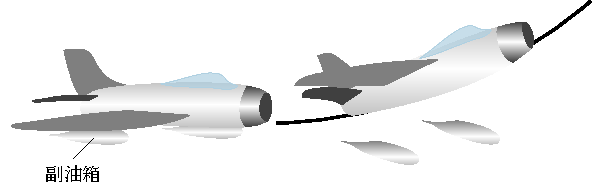
\includegraphics{fig/A/3-2.pdf}
    \caption{歼击机在战斗前抛掉副油箱}\label{fig_A_3-2}
\end{figure}

惯性的大小在实际中是经常要加以考虑的.当我们要求物体的运动状态容易改变时,应该尽可能减小物体的质量.
歼击机的质量比运输机、轰炸机小得多,在战斗前还要抛掉副油箱(图~\ref{fig_A_3-2}),以进一步减小质量,就是为了提高歼击机的灵活性.相反,当我们要求物体的运动状态不易改变时,应该尽可能增大物体的质量.
电动抽水站的电动机和水泵都固定在很重的机座上,就是要增大它们的质量,以尽量减小它们的振动
或避免因意外的碰撞而移动.

那么,力、质量和加速度之间的关系是怎样的呢?下面我们用实验研究这个问题.


\section{加速度和力的关系}
质量一定时加速度和力的关系是怎样的呢?现在随同老师一起做实验来探讨这个问题.

实验装置如图~\ref{fig_A_3-3} 所示,研究对象是图中所示的小车.小车放在光滑的平面上,前端拴着细绳,细绳跨过定滑轮,下面吊着一个砂桶,桶内装砂.
当砂和砂桶的总质量远小于小车的总质量时,小车所受的拉力可以认为等于砂和砂桶的总
重量.因此,用天平称出砂和砂桶的总质量,算出它们的总重量,就得到小车所受的拉力.小车的后面固定一条穿过打点计时器的纸带,随着小车的运动,打点计时器在纸带上打下一列小点,把小车的运动情况记录下来.

\begin{figure}[htp]
    \centering
    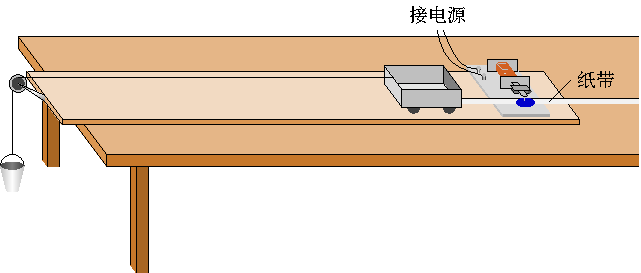
\includegraphics{fig/A/3-3.pdf}
    \caption{研究牛顿第二定律的实验装置}\label{fig_A_3-3}
\end{figure}

每次实验中小车所受的拉力都是恒定的,小车在恒力的作用下,运动情况是怎样的呢?取下纸带,用实验七中所讲的方法来判断小车是否做匀变速运动.
实验结果表明:在恒力的作用下,物体做匀变速运动;也就是说,作用力恒定时,加速度是恒定的.
课后同学们可以根据自己实验的记录纸带,来
判断小车是否做匀变速运动.

在这个实验中还可以进一步求出加速度的大小.加速度的大小可以用实验七中所讲的利用速度图象来求,也可以用下述方法来求.
在纸带上的不同部位分别选取几段距离,用实验七的方法分别求出各段的初速度$v_0$和末速度$v_t$,利用公式$a=(v_t-v_0)/t$分别求出各段的加速度,然后算出平均值作
为小车在整个运动过程中的加速度.课后同学们可以根据自己实验的记录纸带算出小车的加速度.

现在来研究加速度和力的关系.保持小车的质量,改变砂桶里的砂量,再做几次实验.在课后根据记录纸带把各次实验中测得的力和加速度的数据列表记录下来.
表~\ref{tab_A_3-1} 是我们在实验中得到的数据,作为例子放在这里.


\begin{table}[htbp]
	\centering
	\begin{minipage}[b]{0.45\linewidth}
		\centering
		\begin{tabular}{cc}
			\toprule
			$F$  & $a$ \\
			($\UkgfA$)&($\UmsqA$)\\
			\midrule
			0.020  &  0.193  \\
			0.040  &  0.392  \\
			0.060  &  0.588  \\
			0.080  &  0.775  \\
			0.100  &  0.955  \\
			\bottomrule
		\end{tabular}
		\caption{其中 $\UkgfA$ 
			%(kilogram-force)
			表示千克力}\label{tab_A_3-1}
	\end{minipage}
	\hfil
	\begin{minipage}[b]{0.45\linewidth}
		\centering
		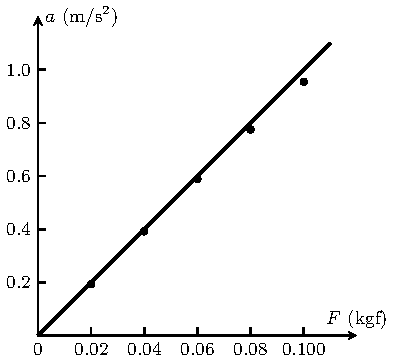
\includegraphics{fig/A/3-4.pdf}
		\captionof{figure}{$a-F$图象}\label{fig_A_3-4}
	\end{minipage}
\end{table}



怎样研究这些数据呢?物理实验中最常用的办法是利用图象.
取横坐标表示力$F$,纵坐标表示加速度$a$,根据实验数据在坐标平面上画出相应的点,
再把这些点连起来作出图象.实验结果表明,得到的图象是一条通过原点的直线(图~\ref{fig_A_3-4}).
这说明物体得到的加速度跟物体所受的外力成正比.课后根据你自己的实验数据作出图象,你得到的是什么图象?




力和加速度都是矢量,它们的方向之间的关系是怎样的呢?在我们的实验中,小车所受拉力的方向和小车的运动方向相同,小车的速度不断增大,加速度的方向也和小车的运动方向相同,由此可知加速度的方向和力的方向是相同的.
运动物体在阻力的作用下速度不断减小,这时阻力的方向和运动方向相反,加速度的方向也和运动方向相反,加速度的方向和阻力的方向仍然相同.
所以,加速度的方向跟引起这个加速度的力的方向是相同的.

总起来说,结论是:

\textbf{对质量相同的物体来说,物体的加速度跟物体所受的外力成正比;加速度的方向和外力的方向相同}.加速度的大小和力的大小的关系,写成公式就是
\[\frac{a_1}{a_2}=\frac{F_1}{F_2} \]
或者
\[a\propto F\]

对于一个确定的物体来说,比如我们从实验确定10牛的力能产生4$\Umsq$的加速度,那么,根据加速度和力成正比,我们就可以知道任何大小的力对这个物体能产生多大的加速度,如15牛的力产生6$\Umsq$的加速度,20牛的力产生8$\Umsq$的加速度,30牛的力产生12$\Umsq$的加速度等等.

\subsection*{练习二}
\begin{enumerate}
	\item 根据你的记录纸带,量出有关数值,计算出每次实验的加速度,列出表格,作出$a-F$图象.
	\item 利用你自己的数据算出每次实验中$a$和$F$的比值,看看这些比值是否大致相同?利用这种办法来研究$a$和$F$的关系,比起用图象来研究,哪种办法方便?
	\item 5牛的力作用在一个物体上,能使它产生2$\Umsq$的加速度,要使它产生5$\Umsq$的加速度,需要多少牛的力?
\end{enumerate}


\section{加速度和质量的关系}
外力一定时,加速度跟质量的关系又是怎样的呢?还是随同老师一起做实验来探讨这个问题.

仍旧用上一节所用的实验装置.保持砂桶里的砂量不变,在小车上放砝码,改变运动物体的质量.
用天平称出小车的质量,加上所放砝码的质量,就是运动物体的质量.

放开小车,用打点计时器在纸带上打点.研究纸带上的点,求出小车的加速度.
改变运动物体的质量,再做几次实验
把各次实验中测得的加速度和质量的数据列表记录下来.
表~\ref{tab_A_3-2} 是我们在实验中测得的数据,作为例子写在这里.

用图象来处理上面的数据.取横坐标表示质量$m$,纵坐
标表示加速度$a$,根据实验数据作出图象.我们看到,画出的图象是一条曲线(图~\ref{fig_A_3-5}).
我们很难从这个图象得到$a$和$m$是什么定量关系.
想想看,怎样才能找出这个定量关系?能不能设法让所画的图象是一条直线呢?
从$a-m$图象可以看出其中一个量增加,另一个量减小,于是猜想$a$和$m$可能是反比关系.
现在改变一下作图方法,取横坐标表示$1/m$,纵坐标表示$a$,看看图象是怎样的.为此需要算出$1/m$的数值.
表~\ref{tab_A_3-3} 是 $1/m$ 和相应的$a$的数据.

\begin{table}[htbp]
	\centering
	\begin{minipage}[b]{0.45\linewidth}
		\centering
		\begin{tabular}{cc}
			\hline
			$m$  & $a$ \\
			($\UkgA$)&($\UmsqA$)\\
			\hline
			0.300  &  1.20  \\
			0.400  &  0.92  \\
			0.500  &  0.81  \\
			0.600  &  0.71  \\
			0.700  &  0.62  \\
			\hline
		\end{tabular}
		\caption{}\label{tab_A_3-2}
	\end{minipage}
	\hfil
	\begin{minipage}[b]{0.45\linewidth}
		\centering
		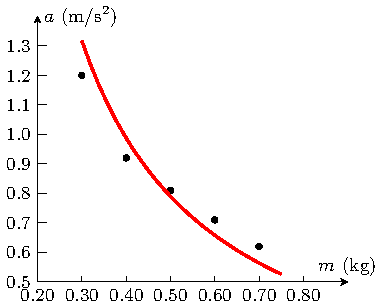
\includegraphics{fig/A/3-5.pdf}
		\captionof{figure}{$a-m$图象}\label{fig_A_3-5}
	\end{minipage}
\end{table}




实验结果表明,得到的图象正是一条通过原点的直线(图~\ref{fig_A_3-6}),这表明我们的猜想是正确的,课后同学们可以根据自己
实验的数据,作出$a-1/m$图象.你得到的图象是一条直线吗?


我们从实验中得到的结论是:\textbf{在相同外力作用下,加速度跟质量成反比}.写成公式就是
\[\frac{a_1}{a_2}=\frac{m_2}{m_1} \]
或者
\[a\propto \frac{1}{m} \]
对于一个确定的力来说,如果我们知道这个力作用在已知质量的物体上产出多大加速度,根据加速度和质量成反比,我们就可以知道这个力对任何质量的物体产生多大加速度.比如一个力作用在1千克的物体上产生10$\Umsq$的加速度,那么,这个力作用在2千克的物体上就产生5$\Umsq$的加速度,作用在5千克的物体上就产生2$\Umsq$的加速度等等.




\begin{table}[htbp]
	\centering
	\begin{minipage}[b]{0.45\linewidth}
		\centering
		\begin{tabular}{cc}
			\hline
			$1/m$  & $a$ \\
			($\Ukg^{-1}$)&($\Umsq$)\\
			\hline
			3.33  &  1.20  \\
			2.50  &  0.92  \\
			2.00  &  0.81  \\
			1.67  &  0.71  \\
			1.43  &  0.62  \\
			\hline
		\end{tabular}
		\caption{}\label{tab_A_3-3}
	\end{minipage}
	\hfil
	\begin{minipage}[b]{0.45\linewidth}
		\centering
		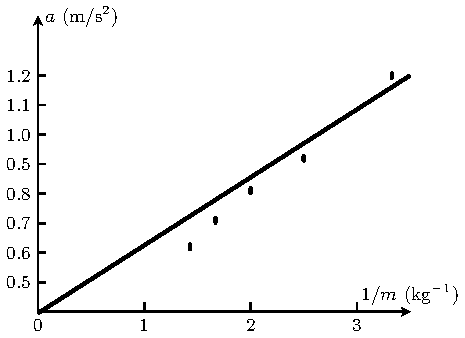
\includegraphics{fig/A/3-6.pdf}
		\captionof{figure}{$a-1/m$图象}\label{fig_A_3-6}
	\end{minipage}
\end{table}





\subsection*{练习三}
\begin{enumerate}
	\item 根据你的记录纸带,量出有关数值,计算出每次实验的加速度,列出表格,作出$a-1/m$图象.
\item 利用你自己的数据算出每次实验中$m$和$a$的乘积,
看看乘积的数值是否大致相同?你由此能得出什么结论?利用这种办法来研究$a$和$m$的关系,比起用图象来研究,哪种办法方便?
\item 你已经用图象研究了$a$和$F$、$a$和$m$的关系,谈谈用图象处理实验数据的好处.
\item 一辆卡车在空载时质量是$3.5\times 10^3$千克,载货时的质量是$6.0\times 10^3$千克.
用同样大小的牵引力,如果空载时使卡车产生1.5$\Umsq$的加速度,载货时产生多大的加速度?(不考虑阻力)
\end{enumerate}

\section{牛顿第二定律}
\subsection{牛顿第二定律及其公式}

总结前两节的结果,关于加速度跟力和质量的关系,我们得到下述结论:

\textbf{物体的加速度跟物体所受的外力成正比,跟物体的质量成反比,加速度的方向和外力的方向相同}.这就是\textbf{牛顿第二定律}.

牛顿第二定律说明,只有受到外力的作用,物体才具有加速度.外力停止作用,加速度随即消失.在持续不断的恒定外力作用下,物体具有持续不断的恒定加速度.外力随着时间而改变,加速度就随着时间而改变.

牛顿第二定律写成公式就是
\[a\propto \frac{F}{m}\quad \text{或者}\quad F\propto ma \]
上式可改写成为等式$F=kma$,其中$k$是比例常数.如果质
量、加速度和力的单位选择适当,可以使$k=1$,公式得到简化.在国际单位制中,质量的单位是千克,加速度的单位是$\UmsqA$,力的单位牛顿就是根据牛顿第二定律规定的:使质量是1千克的物体产生1$\Umsq$的加速度的力,叫做1牛顿.根据这个规定,
\[1 \UN=k[1\Ukg][1\Umsq]=k\times 1[{\rm kg}\cdot \UmsqA]\]
可见,如果$m$,$a$和$F$都用国际单位制的单位,则$k=1$,而且
\[1 \UN=1 \Ukg \cdot \UmsqA\]
牛顿第二定律的公式简化为
\[F=ma\]

等式$F=kma$中的$k$并不是在任何情况下都等于1,例如$m$的单位用千克,$a$的单位用$\UmsqA$,而力的单位用千克力,$k$就不等于1.
这一点我们是应该注意的.


\subsection{力的独立作用原理}
上面讲的是物体受到一个力作用的情况,物体受到几个力的作用时,情况又是怎样的呢?当物体受到几个力的作用时,每个力各自独立地使物体产生一个加速度,就像其他的力不存在一样,这个性质叫做\textbf{力的独立作用原理}.因此物体受到几个力的作用,就产生几个加速度,物体实际的加速度就是这几个加速度的矢量和.
\begin{figure}[htp]
    \centering
    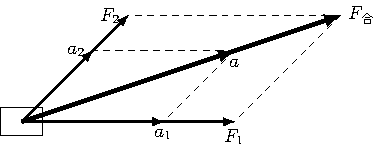
\includegraphics{fig/A/3-7.pdf}
    \caption{}\label{fig_A_3-7}
\end{figure}

如图~\ref{fig_A_3-7} 所示,设物体受到两个力$F_1$和$F_2$的作用,
它们各自独立地产生两个加速度$a_1$和$a_2$,物体实际的加速度$a$就是
按照平行四边形法则求出的这两个加速度的矢量和.
如果再按照平行四边
形法则求出力$F_1$和$F_2$的合力$F_{\text{合}}$,
就可以看出加速度$a$的方向是跟合力$F_{\text{合}}$的方向相同的.
由于$a_1=F_1/m$,$a_2=F_2/m$,所以从图~\ref{fig_A_3-7} 不难得到$a=\frac{F_{\text{合}}}{m}$.可见加速度跟合外力成正比,跟物体的质量成反比.上述结论显然可以推广到物体受到两个以上的力的情况.

这样,我们可以把牛顿第二定律进一步表述如下:

\textbf{物体的加速度跟所受外力的合力成正比,跟物体的质量成反比,加速度的方向跟合外力的方向相同.}

牛顿第二定律的公式可以写成
\[F_{\text{合}}=ma\]


\subsection*{练习四}
\begin{enumerate}
	\item 从牛顿第二定律知道,无论怎样小的力都可以使物体产生加速度,可是我们用力提一个很重的物体时,却提不动它.这跟牛顿第二定律有无矛盾,为什么?
\item 要把一个箱子在地板上从这一端推到另一端,我们在全部时间内都必须用力推它,停止用力,箱子就会停下来.马必须用力拉车,车子才前进,停止用力,车子就会停下来.亚里士多德怎样解释上述现象?根据牛顿运动定律应该怎样解释?
\item 一个物体受到一个逐渐减小的力的作用,力的方向跟速度的方向相同,物体的速度怎样改变?
\item \begin{enumerate}
\item  质量是0.5千克的物体在一个恒力的作用下得到
0.1$\Umsq$的加速度,这个恒力是多大?
\item 10牛的力使一个物体得到2.0$\Umsq$的加速度,这个物体的质量是多大?
\item 质量是0.1千克的物体,在5牛的恒力作用下,得到多大的加速
度?
\end{enumerate}
 \item 质量是1.0千克的物体受到互成30$^\circ$角的两个力的
作用,这两个力都是10牛,这个物体产生的加速度是多大?
\item 下列说法是否正确:
\begin{enumerate}
\item 物体的速度越大,表明物体所受的合外力越大.
\item 根据$F_{\text{合}}=ma$,得到$m=F_{\text{合}}/a$,所以物体的质量跟物
体所受的合外力成正比.
\item 物体所受合外力越大,速度变化越大.
\end{enumerate}


\end{enumerate}

\section{质量和重量}
我们在初中已经学过质量和重量,并且初步讨论了它们
的区别和联系.学过牛顿运动定律之后,对这个问题就会有
进一步的认识了.

我们知道,质量是物体惯性大小的量度.质量是没有方
向的,是标量.
重量是一种力,它是由于地球吸引而产生的,
是使物体产生重力加速度的原因.跟所有的力一样,重力是
有方向的,是矢量.质量和重量的这种不同,在日常现象中也
是能够区别的.例如用手托着一个重球,我们感觉到球对手
有压力,那是因为球有重量的缘故.在水平面上加速这个重
球,我们必须用力,那是因为球有质量的缘故.

如果用$G$表示物体的重量,用$m$表示物体的质量,用$g$表
示重力加速度,那么,根据牛顿第二定律就得到
\[ G=mg\]
这就是质量和重量的关系式.在这个公式中,如果质量用$\UkgA$作单位,重力加速度用$\UmsqA$作单位,重量就要用$\UNA$作单位.
例如物体的质量$m=5.0 \Ukg$,$g=9.8\Umsq$,它的重量
\[G=50 \Ukg \times 9.8\Umsq=49 \UN \]

上述质量和重量的关系式$G=mg$,我们在初中已经见过,
那时我们讲的是$g=9.8 \UNkg $,因为$1\UN=1\Ukg\cdot \UmsqA$,
所以不难证明:$9.8 \UNkg=9.8\Umsq$.


一个物体不论在什么地方质量都是相同的,物体的质量
是一个恒量.实验表明:物体的重量并不是一个恒量;同一
个物体,在地球上不同地方的重量是不同的.
从上式就可以
知道,地球上不同的地方,重力加速度$g$是不同的.
表~\ref{tab_A_3-4} 是一些地点的重力加速度的数值,至于各地的$g$值不同的原因,
将在第\ref{chapter-law-of-universal-gravitation}章加以说明.

应该说明的是,同一物体在地球上不同的地方重量虽然
不同,但相差是很小的,最多只有千分之几.
例如国际标准千克,在北极的重量是9.83216牛,在赤道的重量是9.780304牛.
因此,在一般情况下可以不考虑这个差别,而认为质量是1千
克的物体在地球上任何地方的重量都是9.8牛.这跟在一般
情况下可以不考虑重力加速度$g$在地球上不同地方的差别,
而总是取$g=9.8\Umsq$是一样的.

\begin{table}[htbp]
	\centering
	\caption{重力加速度的数值($\UmsqA$),标准值:$g=9.80665\Umsq$}\label{tab_A_3-4}
	\begin{tabular}{ccc}
		\hline
		地点  &  纬度  &  重力加速度\\
		\hline
		赤道   & $0^\circ$   &  9.780\\
		广州  &  $23^\circ 06'$  &  9.788\\
		武汉  &  $30^\circ 33'$  &  9.794\\
		上海  &  $31^\circ 12'$  & 9.794 \\
		东京  & $35^\circ 43'$   & 9.798 \\
		北京  &  $39^\circ 56'$  & 9.801 \\
		纽约  & $40^\circ 40'$   & 9.803 \\
		莫斯科  &$55^\circ 45'$    & 9.816 \\
		北极  & $90^\circ$   & 9.832 \\
		\hline
	\end{tabular}
\end{table}

在地球上同一个地方,各个物体的重力加速度是相同的.
设在地球上某个地方有两个物体,它们的重量分别是$G_1$和$G_2$,
质量分别是$m_1$和$m_2$,从上述公式得到
\[\frac{G_1}{G_2}=\frac{m_1}{m_2} \]
这就是说,在地球上任一地方,一个物体的重量是另一个的几
倍,它的质量也是另一个的几倍;如果两个物体的重量相等,
它们的质量也相等.天平就是利用这个道理称出物体的质
量的.

由于历史上的原因,人们在日常生活和生产技术中常用
千克力作重量或力的单位.
千克力这个单位原来是指质量为
1千克的物体的重量.但同一物体在地球上不同地方重量不
完全一样,那么,1千克力到底是多大的力呢?为了解决这个
问题,人们规定了千克力的严格定义是
                  \[1 \Ukgf=9.80665\UN\]
为了计算方便,通常取
                    \[1 \Ukgf =9.8 \UN\]
这就是我们在第\ref{chapter-force}章一开始讲过的换算关系.

\subsection*{练习五}
\begin{enumerate}
\item 先后在广州和北京用天平来称量同一个物体,得到
的结果是否相同?如果先后用弹簧秤来称量,得到的结果是否
相同?说明理由.
\item 一个学生认为半块砖的重力加速度是整块砖的重力
加速度的两倍,因为半块砖的质量是整块砖的质量的一半.另
一个学生认为半块砖的重力加速度是整块砖的重力加速度的
一半,因为半块砖的重量是整块砖的重量的一半.他们的说
法对不对?为什么?
\item 北京的重力加速度为980.1$ \Ucmsq $.质量是1千
克的物体在北京的重量是多少牛?
\item 有一架仪器,质量是3.0千克,把它射到月球上,这
架仪器的质量是否改变?它在月球上的重量是多少牛?月球表
面的$g$取1.6$\Umsq$.
\item 仔细看看课文中重力加速度的数值表,从中你可以
得到什么结论?
\item 据说以前有个商人,从荷兰那里把5000吨的货物运
往非洲靠近赤道的某个港口,发现货物少了19吨.在荷兰和
非洲,都是用托盘弹簧秤来称量货物的.你根据书中所列$g$
的数值和荷兰的地理纬度,大致估算一下货物的重量是否会
差这么多.
\end{enumerate}

\section{力学单位制}
\subsection{单位制}
用公式$v=s/t$来求速度的时候,如果位移用米
作单位,时间用秒作单位,求出的速度一定要用$\UmsA$作单位.
同样,用公式$F=ma$来求力的时候,如果质量用千克作单位,
加速度用$\UmsqA$作单位,求出的力一定要用$\UN$作单位.

可见物理公式在确定物理量的数量关系的同时,也确定
了物理量的单位关系.因此,我们可以选定几个物理量的单
位作为基本单位,根据物理公式中其他物理量和这几个物理
量的关系,推导出其他物理量的单位.例如选定位移的单位
(米)和时间的单位(秒),利用公式$v=s/t$
可以推导出速度的单
位($\UmsA$),再利用公式$a=(v_t-v_0)/t$可以推导出加速度的单位
($\UmsqA$).如果再选定质量的单位(千克),利用公式$F=ma$
就可以推导出力的单位($\UkgA\cdot \UmsqA$即牛顿).这些推导出
来的单位叫做\textbf{导出单位}.基本单位和导出单位一起组成了\textbf{单
位制}.

在力学中,我们选定长度、质量和时间三个物理量的单位
作为基本单位,就可以导出其余的物理量的单位.选定这三
个物理量的不同单位,可以组成不同的力学单位制.在国际
单位制中,取米(长度单位)、千克(质量单位)、秒(时间单位)
作为基本单位,本书基本采用这种单位制.

在力学单位制中,除了国际单位制外,现在还有使用厘米$\cdot$
克$\cdot$秒制的,这种单位制取厘米(长度单位)、克(质量单位)、秒(时间单位)作为基本单位.在这种单位制中,速度的单位
是$\UcmsA$,加速度的单位是$\UcmsqA$,力的单位叫做达因.
\[1 \Udyn =1 \Ug\cdot \UcmsqA  \]


\subsection{单位制在物理计算中的作用}
掌握单位制的知识对于物
理计算是很重要的.计算的时候,如果所有的已知量都用同
一种单位制的单位来表示,那么,只要正确地应用物理公式,
计算的结果就总是用这个单位制中的单位来表示的.

现在我们用国际单位制来计算一个题目:一个原来静止
的物体,质量是7.0千克受到14牛的力的作用,求物体的加
速度和5.0秒末的速度.

利用公式$F= ma$求出$a$,再用公式$v_t= at$求出$v_t$:
\[\begin{split}
a&=\frac{F}{m}=\frac{14 \UN}{7.0\Ukg}=\frac{14\Ukg\cdot \UmsqA}{7.0\Ukg}=2.0\Umsq\\
v_t&=at=2.0\Umsq \times 5.0\Us=10\Ums
\end{split} \]

我们看到,题中的已知量都用国际单位制的单位来表示,
得到的答案也是用国际单位制的单位来表示的.既然如此,
解题时就没有必要在计算过程中一一写出各个量的单位,只
在最后标出所求量的单位就行了.今后我们解题一般都用国
际单位制.


\subsection*{练习六}
\begin{enumerate}
\item 在厘米$\cdot$克$\cdot$秒制中,力的单位达因是这样定义的:
使质量是1克的物体产生1$\Ucmsq$的加速度的力,叫做1
\textbf{达因}.试证明: $1\UN=10^5\Udyn$.
\item 有两个力,一个是100达因,一个是20牛,哪个力
大?大的是小的的多少倍?
\item 一个原来静止的物体,质量是600克,受到0.2牛的
力的作用,求物体在3.0秒末的速度.先用国际单位制计算,
再用厘米$\cdot$克$\cdot$秒制计算.
\item 从炮筒射出的炮弹,质量是10千克,速度是$1.0\times 
10^8\Ums$,炮弹在炮筒内运动的时间是$4.0\times 10^{-8}$秒.求火
药爆炸所生气体对炮弹的平均压力.

\end{enumerate}

\section{牛顿运动定律的应用(一)}
    牛顿第二定律确定了力和加速度的关系.因此,已知物
体的受力情况,可以求出加速度.如果再知道物体的初始条
件——初速度和初位置,根据运动学公式就可以求出物体在
任意时刻的位置和速度.这样,已知物体的受力情况,就可以
确定物体的运动情况.这是力学所要解决的一方面的问题.

\begin{example}
一个静止在平面上的物体,质量是2.0千克,
在水平方向受到4.4牛的拉力,物体跟平面的滑动摩擦力是
2.2牛.求物体4.0秒末的速度和4.0秒内发生的位移.
\end{example}

\begin{figure}[htp]
    \centering
    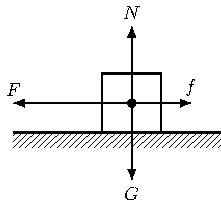
\includegraphics{fig/A/3-8.pdf}
    \caption{}\label{fig_A_3-8}
\end{figure}

\begin{solution}
这个题目就是根据已知的受力情况来求物体的运动情
况.物体受到四个力的作用(图~\ref{fig_A_3-8}):水平拉力$F$,滑动摩擦
力$f$,物体的重量$G$,平面的支持力$N$.物体在竖直方向没有
加速度,重力$a$和支持力$N$大小相等,方向相反,彼此平衡.合
外力就是水平方向的外力$F$和$f$的合力.这里顺便提一下:像
本题这样,物体在水平面上运动,而且水平方向的滑动摩擦
力已经给出,不需要根据竖直方向的压力来求,我们就可以
只考虑水平方向的力,不再考虑竖直方向的彼此平衡的力.



    取水平向左的方向作为正方向,则$F_{\text{合}}=F-f$,根据牛顿
第二定律就有
\[a=\frac{F-f}{m}=\frac{4.4-2.2}{2.0}\Umsq=1.1\Umsq \]
 
 物体的初速度$v_0=0$,将$a$值代入公式
$v_t=at $,$  s=\frac{1}{2}at^2$中即可求出4.0秒末的速度和4.0秒内发生的位移:
\[\begin{split}
v_t&=at=1.1\times 4.0\Ums =4.4\Ums\\
s&=\frac{1}{2}at^2=\frac{1}{2}\times 1.1\times (4.0)^2 \Um=8.8\Um
\end{split} \]
\end{solution}

    算出的$a,v_t,s$都是正值,表示它们的方向都是水平向左
的,与$F$的方向相同,即物体水平向左做初速度为零的匀变速
运动.

\begin{example}
一个滑雪的人从静止开始沿山坡滑下,山坡
的倾角是$30^\circ$,滑雪板和雪地的滑动摩擦系数是0.04.求5.0
秒内滑下的路程.
\end{example}

\begin{figure}[htp]
    \centering
    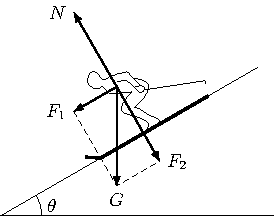
\includegraphics{fig/A/3-9.pdf}
    \caption{}\label{fig_A_3-9}
\end{figure}

\begin{solution}
滑雪的人受到三个力(图~\ref{fig_A_3-9}):重力$G$,山坡的支持力$N$,
滑动摩擦力$f$.把重力$G=mg$沿着平行于山坡方向和垂直于
山坡方向分解成两个力$F_1$和$F_2$,它们的大小是
\[F_1=mg\sin\theta ,\qquad  F_2=mg\cos\theta \]
滑雪人在垂直于山坡方向没有加速度,力$N$和
$F_2$大小相等,方向相反.滑动摩擦力的大小是
\[f=\mu N=\mu mg\cos\theta \]
合外力就是平行于山坡方向的力$F_1$和$f$的合力,
滑雪的人在这个合外力的作用下沿山坡向下做初速度为零的
匀变速运动.

  用公式$F_{\text{合}}=ma$求出$a$,再用公式$s=\frac{1}{2}at^2$,即可求出位
移$s$,即滑下的路程.取与山坡平行而向下的方向作为正方向,
我们得到:
\[\begin{split}
a&=\frac{F_{\text{合}}}{m}=\frac{F_1-f}{m}\\
&=\frac{mg\sin\theta-\mu mg\cos\theta }{m}=g(\sin\theta-\mu \cos\theta)\\
s&=\frac{1}{2}at^2=\frac{1}{2}gt^2(\sin\theta-\mu \cos\theta)\\
&=\frac{1}{2}\times 9.8\times 5.0^2\times \left( \frac{1}{2}-0.04\times \frac{\sqrt{3}}{2}\right)\Um\\
&=57\Um
\end{split} \]


\end{solution}
    
    运动学的任务是描述物体的运动,只说明物体怎样运动,
不讨论物体为什么会做这种或那种运动.学过动力学以后,如
果已知物体的受力情况,我们就可以确定物体的运动情况.这
里还是限于直线运动,下一章就要扩展到曲线运动.牛顿运
动定律同样适用于曲线运动,例如指挥宇宙飞船飞行的科学
工作者,他们知道飞船的受力情况,也知道飞船的初速度和初
位置,因而他们能够确定飞船在任意时刻的位置和速度.他们
解决问题的思路跟我们这里讲的是一样的,只是计算相当复
杂,要用电子计算机进行.


\subsection*{练习七}
\begin{enumerate}
\item 一个质量是100克的运动物体,初速度是0.5$\Ums$,
受到的力是2.0牛,力的方向跟速度方向相同.求3.0秒末的
速度.
\item 一个原来静止的物体受到互成60$^\circ$角的两个力的作
用,这两个力的大小都是50牛,物体的质量是2.0千克,求
3.0秒内物体发生的位移.
\item 一个放在桌面上的木块,质量是0.10千克,在水平
方向受到0.06牛的力,木块和桌面的滑动摩擦力是0.02牛.
求木块通过1.8米所用的时间.
\item 一物体的质量是10千克,在40牛的水平拉力作用
下沿桌面从静止开始运动,物体和桌面的滑动摩擦系数为
0.20.如果在物体运动后的第5秒末把水平拉力撤除,算一
算,一直到运动停止,物体一共走多远.
\item  质量为10千克的物体沿长5米、高2.5米的斜面由
静止匀变速下滑,物体和斜面间的滑动摩擦系数为0.30.物
体的加速度多大?物体从斜面顶端下滑到底端需要多长时间?


\end{enumerate}

\section{牛顿运动定律的应用(二)}
上一节讲了,已知物体的受力情况,可以确定物体的运动
情况.与此相反,如果已知物体的运动情况,根据运动学公式
求出物体的加速度,也可以根据牛顿第二定律确定物体所受
的外力.这是力学所要解决的又一方面的问题.

\begin{example}
1000 吨的列车由车站出发做匀变速运动,列
车经过100秒通过1000米的路程,求机车的牵引力.已知
运动阻力是车重的0.005倍.
\end{example}

\begin{solution}
在这道题目里物体的运动情况是已知的:列车做初速度
为零的匀变速运动,100秒钟通过了1000米的路程,即位移
为1000米.取列车前进的方向为正方向,列车的加速度可以
用公式$s=\frac{1}{2}at^2$求出,即
\[a=\frac{2s}{t^2}=\frac{2\times 1000}{100^2}\Umsq=0.20\Umsq \]

    列车在水平方向受两个力的作用:牵引力$F$和阻力$f$.已
知阻力的大小
\[f=10^6\times 9.8\times 5\times 10^{-3} \UN=4.9\times 10^4 \UN \]
根据
牛顿第二定律$F_{\text{合}}=F-f=ma$就可以求出$F$:
\[\begin{split}
F&=f+ma\\
&=4.9\times 10^4 \UN+10^6\times 0.2 \UN\\
&=2.49\times 10^5\UN
\end{split} \]

$F$为正值表示牵引力方向和所取正方向即列车前进的方
向相同.
\end{solution}


\begin{example}
在汽车中的悬线上挂一个小球,实验表明,当
汽车做匀变速运动时,悬线将不在竖直方向,而与竖直方向成
某一固定角度(图~\ref{fig_A_3-10}).已知小球的质量是30克,汽车的
加速度为5.0$\Umsq$,求悬线对小球的拉力.
\end{example}

\begin{figure}[htp]
    \centering
    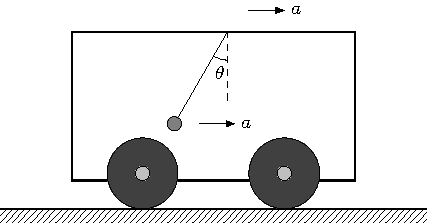
\includegraphics{fig/A/3-10.pdf}
    \caption{}\label{fig_A_3-10}
\end{figure}

\begin{solution}
    在解这个问题时,我们以小球为研究对象,它的运动情况
是已知的.因为小球随着汽车一起做匀变速运动,所以汽车
的加速度$a$就是小球的加速度.小球的受力情况是:受重力
$G$和绳的拉力$T$的作用.小球的受力图如图~\ref{fig_A_3-11} 所示.小
球除了受到这两个力以外,周围再也没有别的物体对小球施
加什么力了.小球的加速度$a$正是由于$G$和$T$这两个力的合
力$F$引起的,根据牛顿第二定律知道,这个合力的方向一定
与小球加速度的方向相同,而且$F=ma$.已知合力$F$,又知
道一个分力$G=mg$,利用平行四边形法则不难求出另一个分
力$T$:
\[T^2=F^2+G^2=(ma)^2+(mg)^2 \]
\[\begin{split}
T&=m\sqrt{a^2+g^2}\\
&=0.030\sqrt{5.0^2+9.8^2} \UN=0.33 \UN
\end{split} \]
\end{solution}

\begin{figure}[htp]
    \centering
    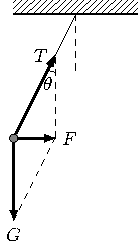
\includegraphics{fig/A/3-11.pdf}
    \caption{}\label{fig_A_3-11}
\end{figure}

    拉力$T$的方向可以用悬线与竖直方向的角度$\theta$表示出
来,角$\theta$不难用\[\tan\theta =\frac{ma}{mg}=\frac{a}{g} \]
求出,请同学们自己算出这个
角度.

    在一些实际问题中,常常需要根据牛顿第二定律从物体
的运动情况来确定力.例如,运动物体所受的线的拉力和支
持物的支持力通常很难用实验来测定,但是,如果知道了物体
的运动情况,算出加速度,根据牛顿第二定律就可以把拉力和
支持力作为未知力求出来.

    在动力学问题中,如果知道物体的受力情况和加速度,也
可以测出物体的质量.这就是说,质量可以用动力学的方法
来测定.本章习题中的第10题,就是用动力学方法测定质量
的一个有趣的题目,希望同学们好好研究一下那个题目.

    从上面两节的例题可以看出,应用牛顿第二定律和运动
学的公式解题时,要首先确定作为研究对象的物体,然后分析
它的受力情况和运动情况,再应用牛顿第二定律和适当的运
动学公式求出未知量.这里,正确分析物体受力情况和运动
情况是解题的关键.

 \subsection*{练习八}
\begin{enumerate}
\item 质量是20吨的车厢以0.2$\Umsq$的加速度前进,运
动的阻力是它的重量的0.02倍,牵引力是多少牛?
\item  列车在水平铁路上行驶,在60秒内速度由82$\Ukmh$增加到54$\Ukmh$,列车的质量是$1.0\times 10^8$吨,机车对
列车的牵引力是$1.5\times 10^5$牛.求列车在运动中所受的阻力.
\item  以1$\Ums$行驶的无轨电车,在关闭电动机以后经
过10秒停下来.电车的质量是$4.0\times 10^3$千克.求电车所受
的阻力.
\item  用弹簧秤拉着一个物体在水平面上做匀速运动,弹
簧秤的读数是0.40牛.然后用弹簧秤拉着这个物体在这个
水平面上做匀变速运动,测得加速度是0.85$\Umsq$,弹簧秤
的读数是2.10牛.这个物体的质量是多大?
\end{enumerate}

\section{超重和失重}
    自从人造地球卫星和宇宙飞船发射成功以来,人们经常
谈到超重和失重,究竟什么是超重和失重呢?

    我们知道,物体的重量是由于地球的吸引而使物体受到
的力.物体的重量可以用弹簧秤称出来.把待测的物体挂在
弹簧秤的下面,当物体和弹簧秤静止时弹簧秤的读数就等于
物体的重量(图~\ref{fig_A_3-12a}).那么,当弹簧秤和物体一起在竖直
方向做加速运动时,弹簧秤的读数还等于物体的重量吗?

    用手提着挂有物体的弹簧秤,使它急剧上升(图~\ref{fig_A_3-12b}),
产生方向向上的加速度.我们看到,这时弹簧秤的读数大于
物体的重量.相反地,如果使它急剧下降(图~\ref{fig_A_3-12c}),产生
方向向下的加速度,弹簧秤的读数就小于物体的重量.怎样
解释这种现象呢?把牛顿第二定律和牛顿第三定律结合起
来,就能解释这种现象了.
\begin{figure}[htp]
    \centering
    \begin{subfigure} {0.3\linewidth} 
		\centering
		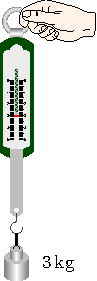
\includegraphics{fig/A/3-12a.pdf} 
		\caption{}\label{fig_A_3-12a} 
	\end{subfigure}
	\hfil
	\begin{subfigure} {0.3\linewidth} 
		\centering
		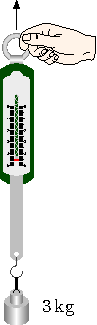
\includegraphics{fig/A/3-12b.pdf} 
		\caption{}\label{fig_A_3-12b} 
	\end{subfigure}
	\hfil
	\begin{subfigure} {0.3\linewidth} 
		\centering
		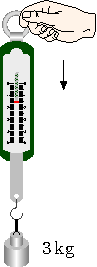
\includegraphics{fig/A/3-12c.pdf} 
		\caption{}\label{fig_A_3-12c} 
	\end{subfigure}
    \caption{}\label{fig_A_3-12}
\end{figure}

    以挂在弹簧秤上的物体作为研究对象,它受到两个力的
作用:重力$G$和弹簧的拉力$T$(图~\ref{fig_A_3-13}).根据牛顿第二定
律知道,正是这两个力的合力使物体做加速运动的.

\begin{figure}[htp]
    \centering
    \begin{subfigure} {0.3\linewidth} 
		\centering
		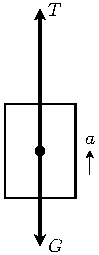
\includegraphics{fig/A/3-13a.pdf} 
		\caption{}\label{fig_A_3-13a} 
	\end{subfigure}
	\hfil
	\begin{subfigure} {0.3\linewidth} 
		\centering
		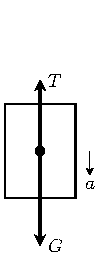
\includegraphics{fig/A/3-13b.pdf} 
		\caption{}\label{fig_A_3-13b} 
	\end{subfigure}
    \caption{}\label{fig_A_3-13}
\end{figure}

    当物体和弹簧秤一起加速上升时,加速度的方向向上(图~\ref{fig_A_3-13a}).取向上的方向为正方向.对物体应用牛顿第二定
律,就有$F_{\text{合}}=T-G=ma$,由此可以求出$T$:
\[ T=G+ma\]

    弹簧秤的读数指的是物体对弹簧的拉力$T'$(图中未画
出),根据牛顿第三定律知道,$T$和$T'$大小相等,方向相反.
所以这时弹簧秤显示出的读数$T'$的大小是$G+ma$,即物体对
弹簧秤的拉力大于物体的重量.跟这类似,如果把物体放在
升降机里的体重计上,当升降机带着物体和体重计一起加速
上升时,物体对体重计的压力的大小也等于$G+ma$,体重计
的读数也大于物体的重量.像这样,当物体存在向上的加速
度时,它对支持物的压力(或对悬挂物的拉力)大于物体的重
量的现象,叫做\textbf{超重现象}.

    当挂着物体的弹簧秤加速下降时,加速度的方向向下(图~\ref{fig_A_3-13b}).取向下的方向为正方向.对物体应用牛顿第二定
律$F_{\text{合}}=G-T=ma$,得到
                               \[T=G-ma\]
    
根据牛顿第三定律知道物体对弹簧的拉力$T'$大小等于
$G-ma$,这时表示物体对弹簧秤拉力的弹簧秤读数小于物体
的重量$G$.同样,当升降机带着物体和体重计一起加速下降
时,体重计的读数也小于物体的重量.像这样,当物体存在向
下的加速度时,它对支持物的压力(或对悬挂物的拉力)小于
物体的重量的现象,叫做\textbf{失重现象}.

\begin{figure}[htp]
    \centering
    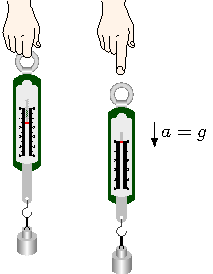
\includegraphics{fig/A/3-14.pdf}
    \caption{}\label{fig_A_3-14}
\end{figure}

    如果把挂着物体的弹簧秤从手中放开(图~\ref{fig_A_3-14}),物体和
弹簧秤将一起自由下落,这时$T=G-mg=0$,弹簧秤的读数
是零.这是容易理解的,因为物体和
弹簧秤一起自由下落,它们之间不发
生相互作用,弹簧不发生形变,所以弹
簧秤的读数为零.同样,当升降机带
着物体和体重计一起以重力加速度$g$
加速下降时,体重计的读数也为零,就
好像物体完全失去了重量一样.物体
对支持物的压力(或对悬挂物的拉力)
等于零的这种状态,叫做完全失重状态.

    应该指出,物体处于超重或失重状态时,地球作用于物体
的重力始终存在,大小也没有发生变化,只是物体对支持物的
压力(或对悬挂物的拉力)发生了变化,看起来好象物体重量
有所增大或减小.


\subsection*{练习九}
\begin{enumerate}
\item 某钢绳所能承受的最大拉力是4.0吨,如果用这条
钢绳使3.5吨的货物匀加速上升,在0.50秒内发生的速度改
变不能超过多大?
\item 升降机以0.30$\Umsq$的加速度竖直减速下降,站在
升降机里60千克的人,对升降机地板的压力是多大?他站在
升降机中的体重计上,体重计表示的他的体重是多大?如果升
降机以相同的加速度竖直减速上升,情况又怎样?在什么情况
下人对地板的压力是零?
\item 弹簧秤上挂一个14千克的物体,在下列各种情况
下,弹簧秤的读数是多大?
\begin{enumerate}
\item 以$28 \Ucmsq$ 的加速度竖直加速上升;
\item 以$10\Ucmsq$的加速度竖直减速上升;
\item 以$10\Ucmsq$的加速度竖直加速下降;
\item 以$28\Ucmsq$的加速度竖直减速下降.
\end{enumerate}
\end{enumerate}

\section{牛顿运动定律的适用范围}
    自从十七世纪以来,以牛顿定律为基础的经典力学不断
发展,取得了巨大的成就.从研究最简单的质点做直线运动
的力学,到研究由若干质点组成的所谓质点系做各种复杂运
动的力学,从研究不变形的物体即所谓刚体的力学,到研究可
变形的连续介质的力学,如流体力学和弹性力学,都属于经典
力学的范围.经典力学在科学研究和生产技术中有广泛的应
用.经典力学和天文学相结合,建立了天体力学,经典力学
和工程实际相结合,建立了各种应用力学,如水力学、材料力
学、结构力学等等.从行星的运动到地面上各种物体的运动;
从大气的流动到地壳的变动;从设计各种机械到拦河筑坝、修
建桥梁和高楼大厦;从人力车、马车的运动到汽车、火车、飞机
等现代交通工具的运动;从抛出石块到发射导弹、人造卫星和
航天飞机——所有这些都服从经典力学的规律.经典力学在
这样广阔领域内用来解决实际问题时得到的结果与实际情况
相符合,证明了牛顿定律的正确性.

    但是,牛顿定律和一切物理定律一样,只具有相对的真理
性,这就是说,牛顿定律也有它的适用范围.

    随着物理学的发展,特别是十九世纪以来电磁理论的发
展,不断发现新的事实,如高速运动的电子的质量随着速度的
增大而增大.这些事实,用经典力学无法加以说明,经典力学
的理论与实验事实之间发生了矛盾.在这种情况下,在二十
世纪初,著名的物理学家爱因斯坦(1879$\sim$1955)提出了狭义
相对论,成为现代物理的开端.狭义相对论从根本上改变了
我们通常对空间和时间的看法,提出了一种新的时空观.从
经典力学看来,物体的长度和时间间隔跟物体运动的速度没
有关系,相对论却指明了它们跟速度的密切关系.相对论还
指出,物体的质量不是固定不变的,它随着物体运动速度的增
大而增大.设$m_0$为物体静止时的质量,那么,物体以速度$v$
运动时,它的质量$m$可以根据相对论力学的公式计算出来.计
算表明,当物体的运动速度$v$接近于光速$c$时,运动物体的质
量$m$远大于它的静止质量$m_0$.例如$v=0.8c$时,$m\approx 1.7m_0$;
$v=0.95c$时,$m\approx 3.1m_0$.这时,经典力学就不再适用了.当物
体的运动速度$v$远小于光速$c$时,虽然运动物体的质量$m$比
它的静止质量$m_0$要大,但相差甚微,可以不予考虑,而认为运
动物体的质量没有改变,经典力学仍旧适用.实际上,太阳系
里的一切宏观物体,如行星、卫星、人造飞船、地球上的各种交
通工具以及我们通常研究的物体,它们的速度都远小于光速,
都显示不出质量随速度而改变的现象.例如,地球的公转速
度$v=3\times 10^4\Ums$,以这个速度运动的物体,它的质量的改
变大约只为静止质量的十万万分之五,这样微小的变化实际
上是无法观测出来的.这就是说,对于太阳系里一切宏观物
体的运动来说,经典力学已经足够准确了.总之,处理低速运
动问题时,经典力学是完全适用的;处理高速运动问题时,必
须用相对论力学.经典力学是相对论力学在低速时良好的近
似.

    经典力学是在研究宏观物体的基础上总结出来的规律.
随着生产和科学技术的发展,十九世纪末和二十世纪初以来,
人们对物质世界的研究深入到原子内部,发现电子、质子、中
子等微观粒子,不仅具有粒子性,而且具有波动性,它们的运
动规律一般不能用牛顿运动定律来说明.二十世纪初期,人
们建立了量子力学,用来描述微观粒子的规律性.关于量子
力学的基本观念,如所谓波粒二象性,到高中三年级再来
学习.

经典力学只适用于解决物体的低速运动问题,不能用来
处理高速运动问题;经典力学只适用于宏观物体,一般不适用
于微观粒子.这就是牛顿定律的适用范围.

\section*{复习题}

\begin{enumerate}
    \item 亚里士多德对力和运动的关系是怎样认识的?他的
    观点有什么错误?
    \item 牛顿第一定律的内容是什么,伽利略的理想实验有
    什么重要意义?
    \item 学习了牛顿第一定律之后,你对力的概念有什么进
    一步的认识?物体运动状态的改变跟什么有关?为什么说质量
    是物体惯性的量度?
    \item 牛顿第二定律的内容是什么?写出它的公式.
    \item 运用牛顿运动定律可以解决哪些方面的问题?你已
    经解过一些动力学的习题,你自己总结一下解题的基本思路
    和步骤.
    \item 质量和重量有什么区别和联系?
    \item 什么叫超重?什么叫失重?
    \item 单位制在物理计算中有什么作用?
    \item 牛顿运动定律的适用范围是什么?
\end{enumerate}


\section*{习题}
\begin{enumerate}
    \item 一个小金属车可以和另外两个相同的小木车在天平
上平衡.用一个力作用在小金属车上,得到2$\Umsq$的加速
度,如果用相同的力作用在一个静止的小木车上,经过2秒,
小木车的速度是多大?

\item  一个质量是$m$克的物体沿着光滑的斜面下滑(不
计滑动摩擦),斜面的倾角是$\theta$.试证明这个物体下滑的加速
度$a=g\sin\theta$.
\item  一个质量是10克的物体沿着光滑的斜面从静止开
始滑下(不计摩擦),开始滑下时的竖直高度是10厘米,斜面
的倾角是30$^\circ$,这个物体滑到斜面末端时的速度是多大?另一
个质量是20克的物体也沿着光滑的斜面从静止开始滑下,开
始滑下时的竖直高度相同,斜面的倾角是45$^\circ$,这个物体滑到
斜面末端时的速度是多大?写出速度$v$的表达式,并说明物体
滑到斜面末端时的速度$v$只跟开始滑下时竖直高度$h$、重力
加速度$g$有关,跟物休的质量$m$、斜面的倾角$\theta$无关.
\item  一个放在水平面上的物体,质量是0.50千克,在水
平方向受到6.0牛的拉力,得到10$\Umsq$的加速度,求这个
物体和平面间的滑动摩擦系数.
\item   质量是2.75吨的载重卡车,在2900牛的牵引力作
用下开上一个山坡,沿山坡每前进1米升高0.05米.卡车由
静止开始前进100米时速度达到36$\Ukmh$.求卡车在前
进中所受的摩擦阻力.
\item  汽车开上一段坡路.汽车的质量是1500千克,发动
机的牵引力是3000牛,摩擦阻力是900牛顿.沿坡路每前进
10米升高2米,坡长282米.汽车用20秒走完这段坡路.求
上坡前的速度和到达坡顶的速度.
\item  有一个质量是3.0千克的木块以速度$v_0$沿光滑的水
平面移动.一个与$v_0$方向相反的18牛的力作用在木块上,
经过一段时间,木块的速度减小到原有速度$v_0$的一半,木块移
动了9.0米的路程.这段时间有多长?$v_0$是多大?
\item  一个物体在两个彼此平衡的力作用下处于静止状
态.现在把其中某一个力逐渐减小到零,这个物体的加速度
和速度的绝对值怎样变化?如果再逐浙把这个力恢复,这个物
体的加速度和速度的绝对值又将怎样变化?
\item  一个放在水平面上的质量是5.0千克的物体,受到
与水平方向成30$^{\circ}$角的斜向上方的拉力作用,物体产生沿水
平方向的加速度是2$\Umsq$.物体跟平面的滑动摩擦系数是
0.1.求拉力是多大?
\item  1966年曾在地球的上空完成了以牛顿第二定律为
基础的测定质量的实验.实验时,用双子星号宇宙飞船$m_1$去
接触正在机道上运行的火箭组$m_2$,接触以后,开动飞船尾部
的推进器,使飞船和大箭组共同加速(图~\ref{fig_A_3-15}).推进器的平均
推力$F$等于595牛,推进器开动7.0
秒钟,测出飞船和火箭组的速度改变
是0.91$\Ums$.已知双子星号宇宙飞
船的质量$m_1=3400\Ukg$.求火箭组的质量$m_2$是多大.
\begin{figure}[htp]
    \centering
    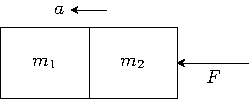
\includegraphics{fig/A/3-15.pdf}
    \caption{}\label{fig_A_3-15}
\end{figure}

\begin{solution}
    推进器的推力使宇宙飞船和火箭组产生的加速度
\[a=\frac{0.91\Ums}{7.0 \Us}=0.13\Umsq \]
根据牛顿第二定律得
\[F=ma=(m_1+m_2)a \]
所以
\[m_2=\frac{F}{a}-m_1=\frac{895}{0.13} \Ukg-3400\Ukg=3500 \Ukg \]
实际上,火箭组的质量已经被独立地测出.实验的目的
是要发展一种技术,找出轨道中另一个国家的人造卫星的未
知质量.事先已测出火箭组的质量为3660千克,因而实验误
差在5\%以内——正好在预期的误差范围之内.
\end{solution}

\item    文艺复兴时代意大利的著名画家和学者达$\cdot$芬奇
提出了如下的原理:
    如果力$F$在时间$t$内使质量是$m$的物体移动一段距离
$s$,那么:
\begin{enumerate}
    \item  相同的力在相同的时间内使质量是一半的物休移动
    $2s$的距离;
\item  或者相同的力在一半的时间内使质量是一半的物体
移动相同的距离;
\item  或者相同的力在两倍的时间内使质量是两倍的物体
移动相同的距离;
\item  或者一半的力在相同的时间内使质量是一半的物体
移动相同的距离;
\item  或者一半的力在相同的时间内使质量相同的物体移
动一半的距离.
\end{enumerate}
    这些原理正确不正确?为什么?

\item   有两个物体,质量为$m_1$和$m_2$,$m_1$
原来静止,$m_2$以速度$v_0$向右运
动(图~\ref{fig_A_3-16}).它们同时开始受到大小
相等、方向与$v_0$相同的恒力$F$的作用,
它们能不能在某一时刻达到相同的速
度?分$m_1<m_2$, $m_1=m_2$, $m_1>m_2$三种情况来讨论.
\begin{figure}[htp]
    \centering
    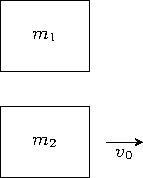
\includegraphics{fig/A/3-16.pdf}
    \caption{}\label{fig_A_3-16}
\end{figure}

\end{enumerate}



